% Options for packages loaded elsewhere
\PassOptionsToPackage{unicode}{hyperref}
\PassOptionsToPackage{hyphens}{url}
%
\documentclass[
]{book}
\usepackage{amsmath,amssymb}
\usepackage{lmodern}
\usepackage{iftex}
\ifPDFTeX
  \usepackage[T1]{fontenc}
  \usepackage[utf8]{inputenc}
  \usepackage{textcomp} % provide euro and other symbols
\else % if luatex or xetex
  \usepackage{unicode-math}
  \defaultfontfeatures{Scale=MatchLowercase}
  \defaultfontfeatures[\rmfamily]{Ligatures=TeX,Scale=1}
\fi
% Use upquote if available, for straight quotes in verbatim environments
\IfFileExists{upquote.sty}{\usepackage{upquote}}{}
\IfFileExists{microtype.sty}{% use microtype if available
  \usepackage[]{microtype}
  \UseMicrotypeSet[protrusion]{basicmath} % disable protrusion for tt fonts
}{}
\makeatletter
\@ifundefined{KOMAClassName}{% if non-KOMA class
  \IfFileExists{parskip.sty}{%
    \usepackage{parskip}
  }{% else
    \setlength{\parindent}{0pt}
    \setlength{\parskip}{6pt plus 2pt minus 1pt}}
}{% if KOMA class
  \KOMAoptions{parskip=half}}
\makeatother
\usepackage{xcolor}
\usepackage{longtable,booktabs,array}
\usepackage{calc} % for calculating minipage widths
% Correct order of tables after \paragraph or \subparagraph
\usepackage{etoolbox}
\makeatletter
\patchcmd\longtable{\par}{\if@noskipsec\mbox{}\fi\par}{}{}
\makeatother
% Allow footnotes in longtable head/foot
\IfFileExists{footnotehyper.sty}{\usepackage{footnotehyper}}{\usepackage{footnote}}
\makesavenoteenv{longtable}
\usepackage{graphicx}
\makeatletter
\def\maxwidth{\ifdim\Gin@nat@width>\linewidth\linewidth\else\Gin@nat@width\fi}
\def\maxheight{\ifdim\Gin@nat@height>\textheight\textheight\else\Gin@nat@height\fi}
\makeatother
% Scale images if necessary, so that they will not overflow the page
% margins by default, and it is still possible to overwrite the defaults
% using explicit options in \includegraphics[width, height, ...]{}
\setkeys{Gin}{width=\maxwidth,height=\maxheight,keepaspectratio}
% Set default figure placement to htbp
\makeatletter
\def\fps@figure{htbp}
\makeatother
\setlength{\emergencystretch}{3em} % prevent overfull lines
\providecommand{\tightlist}{%
  \setlength{\itemsep}{0pt}\setlength{\parskip}{0pt}}
\setcounter{secnumdepth}{5}
\usepackage{booktabs}
\ifLuaTeX
  \usepackage{selnolig}  % disable illegal ligatures
\fi
\usepackage[]{natbib}
\bibliographystyle{plainnat}
\IfFileExists{bookmark.sty}{\usepackage{bookmark}}{\usepackage{hyperref}}
\IfFileExists{xurl.sty}{\usepackage{xurl}}{} % add URL line breaks if available
\urlstyle{same} % disable monospaced font for URLs
\hypersetup{
  pdftitle={A First Course in Probability and Statistics},
  pdfauthor={Nick Syring},
  hidelinks,
  pdfcreator={LaTeX via pandoc}}

\title{A First Course in Probability and Statistics}
\author{Nick Syring}
\date{2022-08-26}

\begin{document}
\maketitle

{
\setcounter{tocdepth}{1}
\tableofcontents
}
\hypertarget{about}{%
\chapter{About}\label{about}}

This is a collection of notes intended for students studying probability and statistics at the advanced undergraduate level at Iowa State University. Specifically, these notes are modeled after course notes for STAT 588, 341, and 342. This site is a work in progress.

Some relevant textbook references include John E. Freund's Mathematical Statistics with Applications by Miller and Miller, or Modern Mathematical Statistics with Applications by Devore and Berk, although many books on this material are available.

\hypertarget{data-analysis-and-statistical-inference}{%
\chapter{Data Analysis and Statistical Inference}\label{data-analysis-and-statistical-inference}}

In this first chapter we define and discuss some important concepts regarding data and scientific investigation.

\hypertarget{data-experiments-and-studies}{%
\section{Data, Experiments, and Studies}\label{data-experiments-and-studies}}

We encounter numerical summaries of information constantly in our everyday lives and sort through these in order to make all sorts of decisions. In this section we will formalize the concept of \emph{data} connected to scientific study. Broadly speaking, data is anything we observe that is relevant to answering a question of interest, i.e., data is tacitly assumed to be informative about the question.

Three types of studies in which data are collected and analyzed are in designed, interventional experiments, observational studies, and exploratory studies. The following illustrations help to differentiate these two types of studies. One difference we will see is all about timing---experiments start with a question of interest and then are designed to answer the question. Exploratory data analysis is often done using data collected with no particular question in mind, or some other question besides the current one. Another difference is that experiments require interventions---imposed changes of behavior or conditions on the individuals in the experiment---while observational studies do not include such interventions.

\hypertarget{james-linds-scurvy-trial}{%
\subsection{James Lind's Scurvy Trial}\label{james-linds-scurvy-trial}}

Clinical trials are familiar designed, interventional experiments. A famous, early example is James Lind's Scurvy trial. Lind was a doctor aboard a British ship. Several sailors with him were suffering from scurvy. He selected 12 sailors in similar, poor condition, and assigned to pairs of them 6 different treatments (the intervention). The two who received oranges and lemons to eat recovered fully; those who received apple cider fared next best. Lind specifically wanted to understand which treatments would be most effective at curing scurvy and planned an experiment to answer his question. His selection of like sailors and random, paired treatment assignment constitute early examples of randomization and control in experimental design.

\hypertarget{framingham-heart-study}{%
\subsection{Framingham Heart Study}\label{framingham-heart-study}}

Named for Framingham, Massachusetts, where the participants were first recruited, this was a long-running observational study of Americans aimed at understanding risks associated with heart disease. Participants agreed to medical testing every 3-5 years, from which the study researchers concluded a number of important findings, such as cigarette smoking substantially increases the risk of heart disease. There are no interventions; the researchers simply observe the patients and make conclusions based on how the patients choose to live, e.g., tobacco use.

\hypertarget{harris-bank-sex-pay-study}{%
\subsection{Harris Bank Sex Pay Study}\label{harris-bank-sex-pay-study}}

93 salaries of entry-level clerical workers who started working at Harris Bank between 1969 and 1971 show men were paid more than women. (From The Statistical Sleuth, reproduced from ``Harris Trust and Savings Bank: An Analysis of Employee Compensation'' (1979), Report 7946,Center for Mathematical Studies in Business and Economics, University of Chicago Graduate School of Business.)

\hypertarget{large-aggregated-data-sets}{%
\subsection{Large, Aggregated Data Sets}\label{large-aggregated-data-sets}}

There are now many large ``data sets'' recording all sorts of information about consumers, e.g., data obtained by Google and other technology companies whenever consumers use their sites, apps, or devices. There are many potential use cases for such information; for instance, such data has proven helpful for targeted marketing of specific products. Such applications may be termed exploratory research---these are characterized, in part, by exploration/examination of data that was originally collected for some other purpose. In other words, the ``data'' was collected with either no question or some other question in mind.

\hypertarget{study-concepts}{%
\subsection{Study Concepts}\label{study-concepts}}

The above examples illustrate several key concepts related to scientific studies.

\begin{itemize}
\tightlist
\item
  Research question - There is always a reason researchers go to the trouble of collecting and analysing data; they have an important question they want to answer. For example, what can sailors do to prevent scurvy?
\item
  Experimental units/Subjects - the research question usually references people, things, animals, or some other entity that can be studied in order to answer the question. When these are observed and measured then they are called experimental units or subjects. In the context of interventional experiments these usually refer to the units of randomization; see below.
\item
  Data - we are inundated with information, numbers, figures, and graphs in our everyday lives. Is this data? Anything information gathered to answer a particular research question can be considered data. Relevancy to a research question is key.
\item
  Intervention - When James Lind gave different foods to sick sailors he was making an intervention, and his goal was to study the effect of his interventions on the sailors well-being. Experiments include one or more interventions, whereas observational studies do not feature any interventions on the part of the researcher.
\item
  Randomization - When researchers intervene, they should apply their interventions randomly with respect to subjects. In experiments the experimental units are the entities that are randomized and given interventions.
\item
  Response/outcome variables - studies often measure multiple variables and study relationships between them. Typically the researchers expect one variable is affected by another. The response, or outcome---like the health of sailors, or pay of workers---is the variable being affected by the intervention in an experiment or by another, independent variable in an observational study.
\item
  Control - Researchers should try to limit the effects of variables on the response that are not of interest to the study. For example, in the gender pay study, the researchers studied only entry-level workers. They \emph{controlled} for prior experience to better isolate potential sex effects on pay.
\end{itemize}

\hypertarget{randomization-control-and-causation}{%
\subsection{Randomization, control, and causation}\label{randomization-control-and-causation}}

In experiments the researcher performs one or more interventions---such as giving patients cider versus citrus fruits in Lind's scurvy trial. The principle of \emph{randomization} asserts that interventions in experiments should be assigned to experimental units randomly. When experimental units are heterogeneous---not all the same---it stands to reason that some of their differences apart from the intervention may impact the response to the experiment recorded by the researcher. Randomization is a way to even out these heterogeneities between groups receiving different interventions. That way, it is the intervention, rather than some other difference, which is responsible for substantially different outcomes. Randomization systematically accounts for heterogeneities, but the extent to which it works depends on the number of experimental units, the number of groups being randomized, and the presence of one or more important heterogeneities. For examples, consider the following:
1. Suppose in ten experimental units there is one unobserved, dichotomous trait that affects the experimental response. Three of the ten have version ``0'' of the trait and 7 have version ``1''. Randomly split the ten into two groups of five, each group to receive a different intervention. The chance all three end up in the same group is 1/6, not ignorably small\ldots{}
2. On the other hand, suppose there are 100 experimental units, half have trait ``0'' and half trait ``1''. The chance at least 35 of either trait type end up in the same one half random split is \(\approx 0\).\\
Generally when an intervention is randomized over experimental units we interpret any significant difference in outcome/response between intervenion groups as having been \emph{caused} by the intervention itself, as opposed to some other unobserved characteristic---these are sometimes called \emph{lurking variables} or \emph{confounding variables}. But, randomization is not foolproof; small sample sizes (few experimental units) and/or the presence of many confounding variables can reduce the effectiveness of randomization.

When the researcher knows about potential confounders ahead of time, the principle of \emph{blocking} says experimental units should be representatively divided with respect to intervention across values of this variable. For example, if experimental units are humans both young and old, then the different interventions should be applied to equal numbers of young and old people. One way to accomplish this is to let age group be a \emph{blocking factor}. In the case of a dichotomous intervention this means half of the old people will be randomly assigned to one intervention and half of the young people will be randomly assigned to one intervention---as opposed to randomly assigning half of all the experimental units to one intervention.

The principle of \emph{control} states that intervention groups should be made as homogeneous as possible. When experiments are well-controlled researchers often assume that they can determine \emph{causation}, and any observed differences in experimental outcome between intervention groups can be attributed to the intervention. Of course, as mentioned above, the ability of an experiment to determine causation is not all or nothing; rather, it depends on unknowns. Nevertheless, stronger controls make the results of experiments more trustworthy, and less likely to be caused by confounding variables.

Non-interventional, observational studies are not used to establish causative relationships. Rather, we say such studies establish \emph{associations} between variables. For example, in the Framingham study, the researchers did not randomly assign individuals to groups of tobacco-users and non-users. Even though these days the evidence is quite strong that tobacco use causes heart disease, the bar for such a claim is much higher when the variable of interest---tobacco use---cannot be randomly assigned to experimental units. That's not to say elements of control cannot be used. For instance, if enough data is collected, it is possible to compare tobacco-users and non-users with nearly the same ages, sexes, incomes, education, living in the same zip codes, etc. The more potential confounders are explicitly controlled, the closer such an observational study comes to a randomized experiment.

\hypertarget{populations-and-scope-of-inference}{%
\subsection{Populations and scope of inference}\label{populations-and-scope-of-inference}}

Whether conducting an experiment or collecting observational data, the units/subjects have to come from somewhere. The \emph{population} refers to the set of all possible subjects---it may be finite or infinite, and it may be concrete or hypothetical. For examples, the population of current Iowa State undergraduates is well-defined, whereas the population of mouse kidney cells exists in a hypothetical sense. \emph{Sampling} describes how subjects are obtained from the population for observation. \emph{Random sampling} is any scheme involving selecting a subset of subjects from a larger group in some random fashion. A \emph{simple random sample} of size \(n\) is obtained when every subset of \(n\) subjects from a total group is equally likely to be selected. Other types of random selection are possible, but we won't often consider these:
- \emph{stratified random sampling} obtains when simple random samples from separate groups/strata are combined, e.g., a 50/50 random sample stratified by male/female can be formed by taking a simple random sample of ten males and a simple random sample of 10 females from a group of 50 males and 50 females
- \emph{cluster random sampling} obtains when a larger group is subdivided into smaller groups and subgroups are selected at random, e.g., a cluster random sample of Iowa high schoolers can be obtained by choosing all high schoolers who attend one of a simple random sample of Iowa high schools.

Generally, conclusions about subjects in the study---whether it is an experiment or an observational study---may be assumed to hold for the wider population as a whole when the subjects are chosen randomly. The details of this \emph{generalizability} of results depend on the type of random sampling conducted; we'll focus on the case of simple random sampling specifically. On the other hand, when subjects are not randomly sampled from the population, study results cannot be generalized back to the population. The reason is that the lack of randomness in selection implies some subsets of the population are more or less likely to be present in the sample of subjects observed, hence, that sample is not necessarily \emph{representative} of the population. For an extreme example, consider a population of both young and old people and an experiment studying the effects of Covid-19. It's well-known Covid-19 is much more harmful to old people compared to young people. So this is a potential confounder. If we select only young people to study, then we certainly cannot claim the results would be similar had we studied both young and old people.

Non-random sampling schemes are quite common because they are usually easier and cheaper to implement than random sampling schemes. A \emph{convenience sample} is just what it sounds like---a rule that selects subjects that are easy to select---such as conducting a poll of your closest friends. When a non-random sample is used, remember that the results cannot be interpreted beyond the group subjects that were observed.

Sometimes a researcher intends to study one population, but obtains data from another population. This mismatch is important to identify as it can cause bias---which simply means the answer to the researcher's question is different for the population for which data is observed compared to the intended population. As in the extreme example above, effects of Covid-19 are different in old and young populations, so the results from an experiment studying only the young are biased when viewed from the perspective of the population of old and young combined.

\hypertarget{data-summaries}{%
\section{Data Summaries}\label{data-summaries}}

Data may take on many forms including sound waves, images comprised of pixels/voxels, and graphs of functions/surfaces. We will almost exclusively consider data that may be represented in a tabulated format, like the following data on weights of chickens.

\begin{verbatim}
##   weight Time Chick Diet
## 1     42    0     1    1
## 2     51    2     1    1
## 3     59    4     1    1
## 4     64    6     1    1
## 5     76    8     1    1
## 6     93   10     1    1
\end{verbatim}

Regardless of the type of data, few users can make sense of all the data at once; rather, we need data summaries---numbers or plots that point out important features of the whole data set.

\hypertarget{numerical-summaries}{%
\subsection{Numerical Summaries}\label{numerical-summaries}}

We briefly describe summaries for categorical and numerical, continuous data.

Suppose a variable \(X\) takes categorical values, e.g., \(X\in\{0,1,2,3\}\). A data set consisting of observed \(x\) values, may be summarized by tabulating proportions, i.e., of 100 observations, 0.41 were \(x=0\), 0.29 were \(x = 1\), 0.17 were \(x = 2\) and 0.13 were \(x=3\). Binary or dichotomous variables may be also be summarized by odds and odds ratios. Suppose \(Y\in\{0,1\}\). The observations \(y_1, \ldots, y_n\) may be summarized by saying \(60\%\) were \(y=1\) versus \(40\%\) \(y=0\) or, equivalently, the observed odds of \(y=1\) was \(0.6/0.4 = 1.5\). Suppose response \(Y\) is \emph{blocked} by another dichotomous variable, say, undergraduate versus graduate status, and suppose the observed odds for undergraduates is 1.5 while the observed odds for graduates is 0.8. Then, the observed odds ratio for undergraduates versus graduates is 1.5/0.8 = 1.875.

In contrast to categorical data, continuous data takes values in the real numbers \(\mathbb{R}\) or some interval of real numbers. Most numerical summaries of continuous variables either measure location or dispersion. Location refers, in one way or another, to a typical or average value while dispersion refers to the spread of the values. Common measures of location are the mean, median, and trimmed mean:

\begin{itemize}
\tightlist
\item
  The mean of \(x_1, \ldots, x_n\) is \(\overline x = n^{-1}\sum_{i=1}^n x_i\).
\item
  The median is denoted \(\tilde x\). Sort the \(x\)'s from least to greatest labeling them as \(x_{(1)}, \ldots, x_{(n)}\). Then, \(\tilde x = x_{(\frac{n+1}{2})}\) if \(n\) is odd and \(\tilde x = \tfrac12\left(x_{(\frac{n}{2})} + x_{(\frac{n}{2}+1)}\right)\) if \(n\) is even.
\item
  The \(\alpha\%\) trimmed mean is the mean of the remaining \(x\) values after ignoring the smallest and largest \(\alpha\%\) of values. Roughly, the \(\alpha\%\) trimmed mean averages \(x_{(1+\alpha n)},\ldots, x_{n - \alpha n - 1}\).
\item
  Besides the median, we may be interested in ``locations'' besides the center, and these could be summarized using quantiles. Observed quantiles may be defined in a number of ways. One definition says the \(\alpha\in(0,1)\) quantile is the smallest observed \(x\) value such that at least \(\alpha\%\) of observed \(x\) values are no more than \(x\).
\end{itemize}

Common measures of dispersion include the variance and standard deviation, the range, and the interquartile range:

\begin{itemize}
\tightlist
\item
  The observed variance of \(x_1, \ldots, x_n\) is given by \(\tfrac{1}{n-1}\sum_{i=1}^n(x_i - \overline x)^2\) and may be equivalently computed as \(\tfrac{1}{n-1}\left\{\sum_{i=1}^n (x_i^2) - n\overline x^2\right\}\).\\
\item
  In the calculation of variance the \(x\) values are squared, which means the variance has units equal to the squared units of \(x\); that is, if \(x\) is measured in millimeters then its variance is measured in millimeters squared, or, e.g., dollars then dollars squared. Often the squared units are difficult to interpret. Instead, we define the standard deviation as the square root of the variance, which shares the units of the observed \(x\) variable.\\
\item
  The range is the difference between maximum and minimum values, i.e., \(x_{(n)} - x_{(1)}\).
\item
  The interquartile range (IQR) is the difference between the \(0.75\) and \(0.25\) quantiles.
\end{itemize}

\hypertarget{visual-summaries}{%
\subsection{Visual Summaries}\label{visual-summaries}}

Plots and graphs can also be used to summarize a data set or particular observed variable. Three plots we will use extensively in the course are the scatterplot, histogram, and quantile-quantile (qq) plot.

\begin{itemize}
\item
  For paired observations of two variables \((x_i, y_i), \,\,i = 1, \ldots, n\) a scatterplot displays \((x_i, y_i)\) in the xy-plane. For example, see the plot of a chicken's weight versus time from the tabulated data set above. Scatterplots are useful for assessing relationships between variables. For example, the chick's weight increases with time, maybe in a linear or slightly quadratic fashion.
  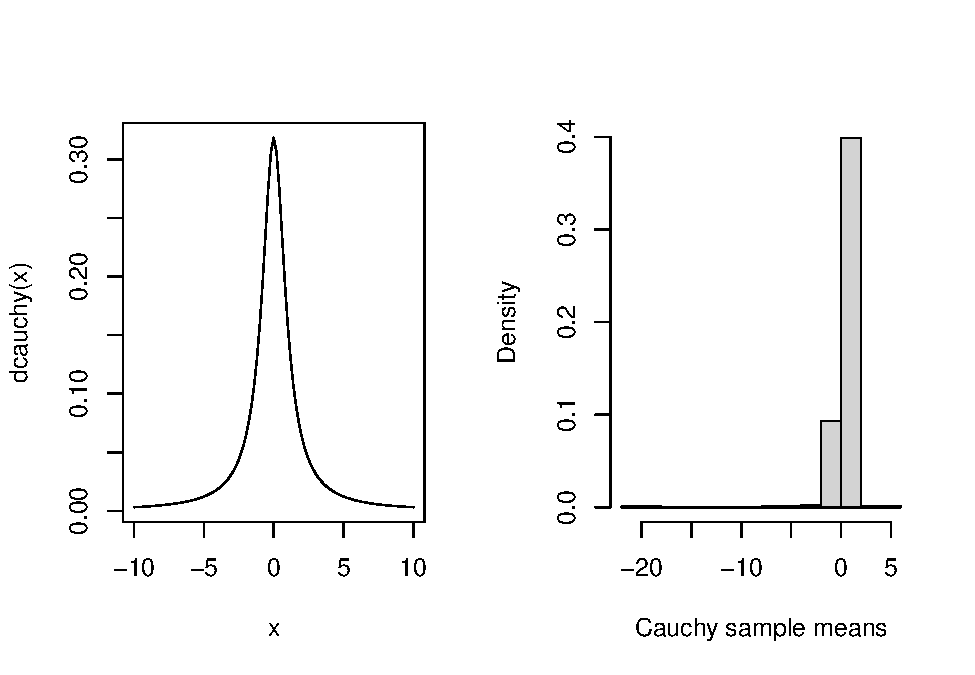
\includegraphics{01-intro_files/figure-latex/unnamed-chunk-2-1.pdf}
\item
  For a single variable a histogram summarizes the distribution of its observed values by counting the numer of observations in different intervals (buckets) of values. Keep in mind that histograms with different choices of buckets may look very different. Check out this histogram of ``Time 0'' weights of all 23 chicks.
  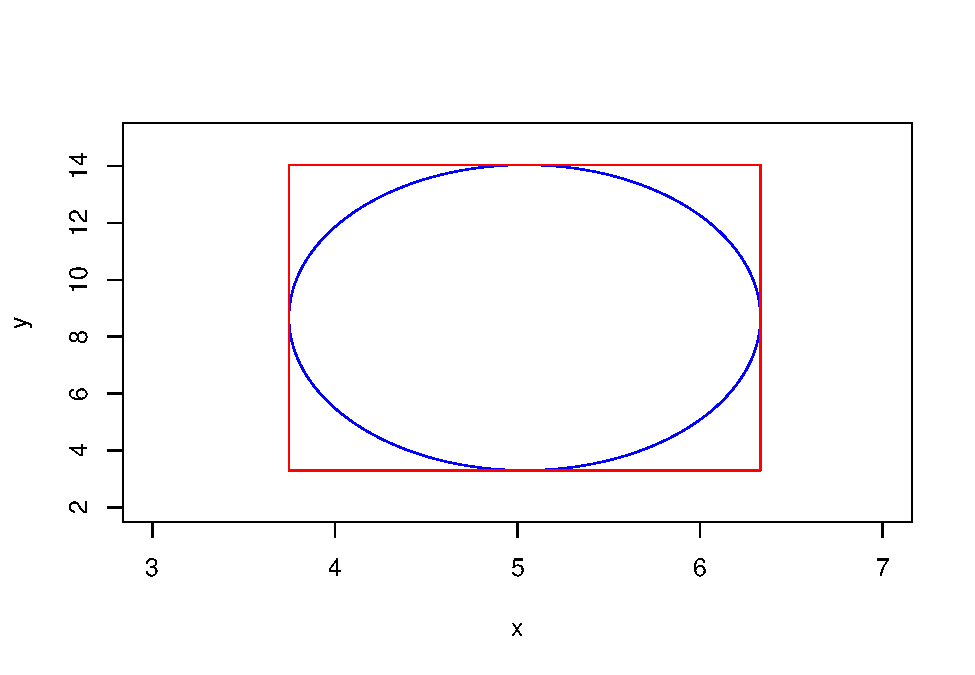
\includegraphics{01-intro_files/figure-latex/unnamed-chunk-3-1.pdf}
\item
  A qq-plot compares the shape of a distribution of observed values to another known distribution, often the standard normal distribution. For example, make the standardizing transformation \((x_i - \overline x) / \hat\sigma_x\) where \(x_i\) is the Time 0 weight of chick \(i\), \(\overline x\) is the observed mean and \(\hat\sigma_x\) is the observed standard deviation of those values. Compute the \(\alpha\) quantile of these values or several \(\alpha\) values in \((0,1)\) along with the corresponding standard normal quantiles (z-scores). Plot the pairs of \(\alpha\) quantiles in the xy-plane. If the standardized weights are approximately normal, then the points should lie approximately on the line \(y=x\). Note that extreme quantiles are always less reliably estimated, so it is typical for the ends of the ``line'' to fray up or down from the diagonal.
\end{itemize}

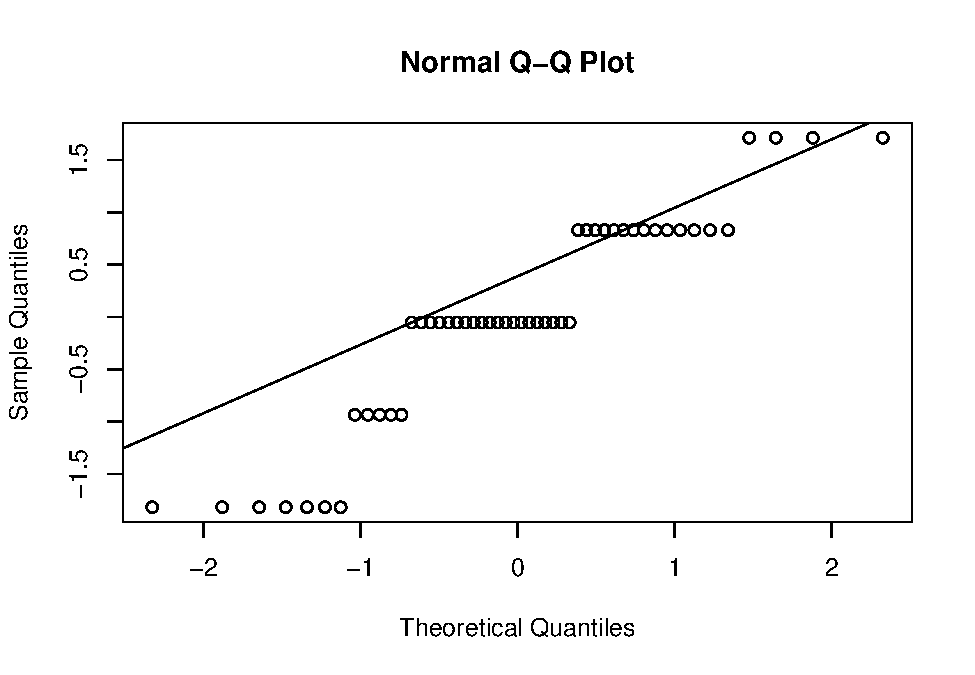
\includegraphics{01-intro_files/figure-latex/unnamed-chunk-4-1.pdf}

\hypertarget{statistical-inference}{%
\section{Statistical Inference}\label{statistical-inference}}

Summarizing data sets is important because no one can make sense of more than a few numbers at a time. But, data summaries cannot by themselves answer our research questions. That is because data summaries only say something about the particular data set we observe, while our research questions concern the whole population. Recall, a major aim of experimentation is generalizing from observations to population. When we make such generalizations we often refer to them as \emph{inferences}; and, statistical inferences are characterized by their careful treatment of statistical concepts, such as hypotheses, and Type 1 and 2 errors, which we discuss below.

A hypothesis is a claim or assertion about a population. These may be simple, i.e., ``the population mean is 5'', or more complex, like ``the population distribution of values is equivalent to a Normal probability distribution''. Notice that both of these statements are either true or false, yes or no. A hypothesis then may be called the ``null hypothesis'', and its complement (opposite) the alternative hypothesis. Which is which depends on the context. We make educated guesses about the truthfulness of a null hypothesis based on observations/data. Our educated guesses may be right or wrong, but we will never know because we will never ``see'' the whole population. If we reject the null hypothesis as false when it really is true, then we make a Type 1 error. The opposite, keeping the null hypothesis in favor over its alternative, when it is actually false, is a Type 2 error. Ideally, we would make no errors, but that's not possible. In fact, the two errors have an inverse relation. For example, if we adopt the rule that we always reject the null hypothesis, then we will necessarily maximize Type 1 errors but have no Type 2 errors. And, if we take the opposite approach, then we maximize Type 2 errors while making no Type 1 errors.

Much of this course will focus on constructing tests of relevant hypotheses with the property that we limit the chance of making a Type 1 error. By chance we refer to the probability distribution of the test outcome induced by random sampling of data from the population. A test that has chance no more than \(\alpha\) of making a Type 1 error is called a ``level \(\alpha\) test of \(H_0\)'', the null hypothesis.

\hypertarget{statistical-estimation}{%
\chapter{Statistical Estimation}\label{statistical-estimation}}

\hypertarget{vocabulary}{%
\section{Vocabulary}\label{vocabulary}}

We consider experiments in which a random sample of observations is taken from a population. The sampling distribution of observations is known up to the value(s) of some \emph{population parameter(s)}. The goal of this chapter is to study \emph{estimation}---approximation of these unknown parameters by \emph{statistics}, functions of the sample data. An \emph{estimator} is the random variable version of a statistic and has a corresponding sampling distribution. By virtue of being called an estimator we assume this statistic is ``close'' to the true parameter value in some sense. An \emph{estimate} is a value of an estimator after the data is collected and the estimator computed; it is a fixed, non-random value.

For example, consider an experiment sampling \(n\) iid random samples from a Normal population with unknown mean \(\mu\) and variance \(1\). Here \(\mu\) is the parameter we wish to estimate. An intuitive estimator is the sample mean statistic \(\overline X_n = n^{-1}\sum_{i=1}^n X_i\). When the data is collected we refer to the calculated sample mean---the estimate of \(\mu\)---as lowercase \(\overline x_n\).

\hypertarget{properties-of-estimators}{%
\section{Properties of Estimators}\label{properties-of-estimators}}

It will become apparent that estimators are not unique---there are very often several seemingly reasonable estimators for a single parameter. Therefore we ought to be concerned with choosing the ``best'' estimator according to some criteria. Different criteria will lead to different ``best'' estimators.

\hypertarget{bias-and-unbiasedness}{%
\subsection{Bias and Unbiasedness}\label{bias-and-unbiasedness}}

Consider a generic parameter denoted \(\theta\) and imagine an estimator for \(\theta\) called \(\hat\theta_n\), which is a statistic and, hence, a random variable. We say \(\hat\theta_n\) is \emph{unbiased} if \(E(\hat\theta_n)=\theta\) where the expectation is taken with respect to the sampling distribution of \(\hat\theta_n\). For example, the sample mean \(\overline X_n\) is unbiased for the population mean \(\mu\) (so long as the population mean exists):
\begin{align*}
E(\overline X_n) &= E\left(n^{-1}\sum_{i=1}^n X_i\right)\\
& = n^{-1}\sum_{i=1}^n E(X_i)\\
& = n^{-1}\sum_{i=1}^n \mu\\
& = \mu.
\end{align*}
An unbiased estimator commits no systematic errors in estimating the parameter. In contrast, a biased estimator of a univariate real-valued parameter systematically underestimates or overestimates the parameter. Consider biased \(\hat\theta_n\) such that \(E(\hat\theta_n) = \theta + 1\). We \textbf{expect} \(\hat\theta_n\) to be 1 more than \(\theta\)---hence we expect it to overestimate.

\hypertarget{minimum-variance-unbiased-estimators}{%
\subsection{Minimum Variance Unbiased Estimators}\label{minimum-variance-unbiased-estimators}}

Besides a finite mean, estimators often have a finite variance. And, intuitively, we would tend to prefer an estimator with low variance to one with high variance, particularly if both are unbiased. If we insist on an unbiased estimator, then the ``best'' unbiased estimator is the unbiased estimator with smallest variance among all unbiased estimators.

It is not obvious how one would find the lowest variance estimator among all unbiased estimators. One result, due to CR Rao and Harald Cramer, provides a lower bound on the variance of an unbiased estimator. This lower bound can be checked by computing the variance of a given unbiased estimator, and, if they match, this implies the given estimator is the MVUE. We describe this procedure below.

Let \(f(x;\theta)\) denote the density of the data and let \(\theta\) denote a univariate parameter. Let \(\ell(x;\theta) := \log(f(x;\theta))\), the natural logarithm of the density. Define the \emph{Fisher Information} for one data point by
\[I(\theta) = E\left[\left(\frac{\partial \ell(x;\theta)}{\partial\theta}\right)^2\right].\]
The Fisher information for a random sample of size \(n\) is \(n\) times \(I(\theta)\). Then, Cramer and Rao showed that if \(\hat\theta_n\) is unbiased, its variance cannot be smaller than
\[V(\hat\theta_n)\geq \left[nI(\theta)\right]^{-1}\]
where \(\theta\) is the true parameter value.

Example: Let \(X_1, \ldots, X_n\) be a random sample from a normal population with variance 1 and mean \(\mu\) and consider the estimator \(\overline X_n\). The logarithm of the density function is
\[\ell(f(x;\mu)) = -\log(\sqrt{2\pi}) - \tfrac12(x - \mu)^2\]
with \(\mu-\)derivative \(x - \mu\). Therefore, the Fisher Information is
\[I(\mu) = E[(X - \mu)^2] = 1\]
since it is, by definition, equal to the variance. The Cramer-Rao lower bound is
\[V(\hat\theta_n)\geq \frac{1}{n},\]
and we know \(V(\overline X_n) = 1/n\) so the sample mean \(\overline X_n\) is, indeed, the MVUE for this experiment.

\hypertarget{mean-squared-error-and-bias-variance-tradeoff}{%
\subsection{Mean Squared Error and Bias-Variance tradeoff}\label{mean-squared-error-and-bias-variance-tradeoff}}

As described above a common strategy is to select an unbiased estimator, preferably one with low (or the lowest) variance. On the other hand, one may prefer a biased estimator over an unbiased one if the bias is low and there is substantial reduction in variance. One way to choose estimators that balance bias and variance is to consider their mean squared error (MSE), defined by
\[MSE(\hat\theta_n) = E[(\hat\theta_n - \theta)^2] = Bias(\theta_n)^2 + V(\hat\theta_n).\]
It is left as an exercise to the reader to show the MSE equals the sum of estimator variance and squared bias. For the above reasons the estimator minimizing the MSE may be preferable even to the MVUE.

Example: Estimation of a normal population variance
The usual variance estimator is the sample variance \(S^2_n = \frac{1}{n-1}\sum_{i=1}^n (X_i - \overline X_n)^2\). It can be checked this estimator is unbiased. And, it is a bit of a pain, but it can be shown that \(V(S_n^2) = \frac{2\sigma^4}{n-1}\). Now, consider an alternative estimator that is a constant multiple of \(S^2_n\), say \(c S_n^2\) for some \(c>0\). The MSE of this estimator is
\begin{align*}
MSE(cS_n^2) &= V(cS_n^2) + Bias(cS_n^2)^2\\
& = c^2\frac{2\sigma^4}{n-1} + [E(cS_n^2) - \sigma^2]^2\\
& = c^2\frac{2\sigma^4}{n-1} + (c\sigma^2 - \sigma^2)^2\\
& = c^2\frac{2\sigma^4}{n-1} + \sigma^4(c-1)^2.
\end{align*}
Differentiate w.r.t. \(c\) to find
\[\frac{\partial MSE}{\partial c} = 2c \frac{2\sigma^4}{n-1} + 2(c-1)\sigma^4.\]
Set this equal to zero and solve for \(c\). We get
\[c = \frac{2\sigma^4}{\frac{4\sigma^4}{n-1} + 2\sigma^4} = \frac{n-1}{2+n-1} = \frac{n-1}{n+1}.\]
This means the minimim MSE estimator (at least among those that are multiples of \(S_n^2\)) is actually \(\frac{1}{n+1}\sum_{i=1}^n (X_i - \overline X_n)^2\).

\hypertarget{consistency}{%
\subsection{Consistency}\label{consistency}}

Besides avoiding systematic estimation errors and having low variance, we would expect that as more and more data is collected an estimator should get better and better---and get ``closer'' to the true parameter, in some sense. This intuition is captured mathematically by \emph{consistency}. An estimator is consistent if for any \(c>0\), however small,
\[\lim_{n\rightarrow \infty} P(|\hat\theta_n-\theta|>c) = 0.\]
Dissecting this definition from the inside out we first note \(|\hat\theta_n - \theta|\) is the random estimation error. Then, \(|\hat\theta_n-\theta|>c\) says the error is at least \(c\). Since the error is a random variable we attach a probability to the chance the error is at least \(c\), which is \(P(|\hat\theta_n-\theta|>c)\). And, consistency says this probability must vanish as we accumulate data. So, the chance of an error of any size \(c\) or bigger vanishes. Taking complements, this is equivalent to saying
\[\lim_{n\rightarrow \infty} P(|\hat\theta_n-\theta|<c) = 1,\]
which means \(\hat\theta_n\) is within \(c\) of \(\theta\) with probability going to 1.

One way to show an estimator is consistent is to show it is unbiased and has variance that vanishes as \(n\rightarrow 0\). One example is the sample mean, which is unbiased and has variance \(\sigma^2/n\). Then, consistency follows by Chebyshev's inequality, which says: for any r.v. \(X\) with finite mean and variance \((\mu, \sigma^2)\),
\[P(|X - \mu|>c)\leq \frac{\sigma^2}{c^2}\]
for any \(c>0\). In the context of estimation, we have
\[P(|\hat\theta_n - E(\hat\theta_n)|>c) \leq \frac{Var(\hat\theta_n)}{c^2}.\]
Now, suppose \(\hat\theta_n\) is unbiased and its variance vanishes in \(n\). Then, the above statement says
\[P(|\hat\theta_n - \theta|>c) \leq s_n.\]
for a sequence \(s_n\) satisfying \(\lim_{n\rightarrow \infty} s_n = 0\). Checking the definition we see this means \(\hat\theta_n\) is consistent. A similar argument can work for biased estimators as well, provided the bias also vanishes as \(n\rightarrow\infty\). Such estimators are called \emph{asymptotically unbiased}. One such example is the minimum MSE estimator of \(\sigma^2\) from the previous section. It has bias \(\sigma^2(\frac{n-1}{n+1}-1)\) which has limit zero.

\hypertarget{finding-estimators---method-of-moments}{%
\section{Finding estimators - Method of Moments}\label{finding-estimators---method-of-moments}}

So far we've discussed desirable properties of estimators but not where these estimators come from. How do we find estimators in the first place? One strategy is based on the fact population parameters often are related to population moments. Then, we can find estimators by replacing population moments by sample moments and referring back to the relationship between the moments and parameters. The simplest example of the method of moments is estimation of the population mean by the sample mean.

Example: Suppose a population is modeled as a Gamma distribution with shape and rate parameters \((\alpha, \beta)\). The population mean is \(\alpha / \beta\) and the population variance is \(\alpha / \beta^2\). This means the population second raw moment is \(\alpha / \beta^2 + (\alpha / \beta)^2\). We can estimate \((\alpha, \beta)\) by matching the sample and population raw moments as follows:
\begin{align*}
n^{-1}\sum_{i=1}^n X_i &= \alpha/\beta^2\\
n^{-1}\sum_{i=1}^n X_i^2 &= \alpha/\beta^2 + (\alpha / \beta)^2.
\end{align*}
Solving the system by substitution we have
\begin{align*}
\hat\alpha = \frac{\hat\mu_2' - \hat\mu_1'}{\hat\mu_1'}\\
\hat \beta = \sqrt{\frac{\hat\mu_2' - \hat\mu_1'}{(\hat\mu_1')^2}},
\end{align*}
where \(\hat\mu_1'\) and \(\hat\mu_2'\) indicate the 1st and second raw sample moments \(n^{-1}\sum_{i=1}^n X_i\) and \(n^{-1}\sum_{i=1}^n X_i^2\).

Example: Suppose we will take a random sample of size \(n\) from a continuous uniform distribution supported on the interval \((a,b)\) where the endpoints are unknown. We know that \(E(X) = \frac{a+b}{2}\) and \(V(X) = \frac{(b-a)^2}{12}\) so that \(E(X^2) = \frac{(b-a)^2}{12} + \frac{(a+b)^2}{4}\). Then, we find estimators for \((a,b)\) by solving
\begin{align*}
n^{-1}\sum_{i=1}^n X_i &= \frac{a+b}{2}\\
n^{-1}\sum_{i=1}^n X_i^2 &= \frac{(b-a)^2}{12} + \frac{(a+b)^2}{4}.
\end{align*}
With some work, you should find \((\hat a, \hat b) = (\hat\mu_1' - \sqrt{3\hat\mu_2'}, \, \hat\mu_1'+\sqrt{3\hat\mu_2'})\). That's not so intuitive\ldots{} What about using the sample minimum and maximum\ldots{}

\hypertarget{method-of-maximum-likelihood}{%
\section{Method of Maximum Likelihood}\label{method-of-maximum-likelihood}}

Again consider a random sample \(X_1, \ldots, X_n\) from a population synonymous with a density function \(f(x;\theta)\) for an unknown parameter \(\theta\). For the time being consider only scalar \(\theta\). The \emph{likelihood function} is the joint PDF of the data viewed as a function of the parameter, and may be treated either as a random function or as a deterministic function depending on whether the data are treates as random variables or as observed values, so pay close attention to the context. For iid data the likelihood can be written
\[L(\theta;X_1, \ldots, X_n) = \prod_{i=1}^n f(X_i;\theta).\]

For the purpose of estimating \(\theta\) we view the likelihood as a deterministic function given observations. Then, it acts as a sort of ``ranking function'' that provides a quantitative comparison of how well different parameter values agree with the observed data. The idea is to select as an estimate the parameter value that maximizes the likelihood/agreement with the data. To explain this concept of agreement with the data a bit more suppose the data come from a discrete population so that \(f(x;\theta)\) is a PMF rather than a density---this makes the interpretation easier. Then \(\prod_{i=1}^n f(X_i;\theta)\) is a the probability of observing the data for a given parameter value \(\theta\). Choosing \(\theta\) to maximize this probability means selecting the distribution that gives the highest probability assignment to the data that was actually observed.

Example: Suppose our random sample comes from an Exponential distribution with rate \(\lambda\). The likelihood function equals
\begin{align*}
L(\lambda, x_1, \ldots, x_n) &= \prod_{i=1}^n \lambda^{-1}e^{-x_i/\lambda}\\
& = \lambda ^{-n}e^{-\tfrac1\lambda\sum_{i=1}^n x_i}.
\end{align*}

Take the first derivative of the likleihood with respect to \(\lambda\):
\[\frac{\partial L}{\partial \lambda} = -n\lambda^{-(n+1)}e^{-\tfrac1\lambda \sum_{i=1}^n x_i} + \lambda^{-n}e^{-\tfrac1\lambda\sum_{i=1}^n x_i}\left(\lambda^{-2}\sum_{i=1}^n x_i\right)\]
Set \(\tfrac{\partial L}{\partial \lambda}\) equal to zero and solve for \(\lambda\) to obtain the MLE:
\begin{align*}
\frac{\partial L}{\partial \lambda} = 0 & \Rightarrow -n\lambda^{-1} + \tfrac{1}{\lambda^2}\sum_{i=1}^n x_i = 0\\
& \Rightarrow n\lambda = \sum_{i=1}^n x_i\\
& \Rightarrow \hat{\theta}_{MLE} = \overline x_n.
\end{align*}

Example: Suppose our random sample comes from a Uniform distribution on the interval \((0,\theta)\). The likelihood function equals
\begin{align*}
L(\lambda, x_1, \ldots, x_n) &= \prod_{i=1}^n \frac{1}{\theta}1(0\leq x_i\leq \theta) \\
& = \theta^{-n}\prod_{i=1}^n 1(0\leq x_i\leq \theta).
\end{align*}

We cannot simply maximize this likelihood function by taking the first derivative because the indicator functions are not everywhere differentiable w.r.t. \(\theta\). Instead, note that the function \(\theta^{-n}\) is monotonically decreasing in \(\theta\); so, this function prefers small \(\theta\). On the other hand, the function \(\prod_{i=1}^n 1(0\leq x_i\leq \theta)\) is constant and equal to 1 so long as \(\theta \geq \max_{i=1, \ldots, n} x_i\); otherwise, this function is zero and so is the likelihood (and the likelihood cannot be less than zero!). This means we should choose \(\theta = \max_{i=1, \ldots, n} x_i\) to maximize the likelihood. Therefore, the MLE of \(\theta\) is \(\hat\theta_{MLE} = max_{i=1, \ldots, n} x_i\).

Multivariate Example: Consider estimation of both the mean and variance parameters of a normal population based on a random sample of size \(n\) denoted \(X^n = (X_1, \ldots, X_n)^\top\). The likelihood is a function of two parameters \((\mu, \sigma^2)\):
\[L(\mu, \sigma^2;X^n) = (2\pi\sigma^2)^{-n/2}\exp\left(-\frac{1}{2\sigma^2}\sum_{i=1}^n (X_i-\mu)^2\right).\]
The loglikelihood is easier to maximize so take the log and find
\[\ell(\mu, \sigma^2;X^n) = -\frac{n}{2}\log (2\pi\sigma^2) -\frac{1}{2\sigma^2}\sum_{i=1}^n (X_i-\mu)^2. \]
To find the MLEs we need to compute the gradient vector:
\begin{align*}
\frac{\partial\ell}{\partial \mu} &= \frac{1}{\sigma^2}\sum_{i=1}^n (X_i-\mu)\\
\frac{\partial\ell}{\partial \sigma^2} &= -\frac{n}{2\sigma^2} + \frac{1}{2\sigma^4}\sum_{i=1}^n (X_i-\mu)^2.
\end{align*}
Setting \(\frac{\partial\ell}{\partial \mu}=0\) we immediately find \(\hat\mu_{MLE} = \overline X_n\). Substituting this estimate for \(\mu\) in the second equation we find \(\hat\sigma^2_{MLE} = \frac{1}{n}\sum_{i=1}^n (X_i-\overline X_n)^2\), the version of the sample variance with denominator \(n\) instead of \(n-1\). The following result says the MLE has variance approximately equal to the reciprocal of the Fisher information when the parameter is a scalar. In the multivariate setting the analogous quantity is the inverse Fisher information matrix, which is the inverse of the expectation of \(-1\) times the matrix of second partial derivatives of the loglikelihood. Let's calculate this variance-covariance matrix next. First, we need to compute the matrix of second partial derivatives of the loglikelihood:\\
\begin{align*}
\frac{\partial^2\ell}{\partial \mu^2} &= -\frac{n}{\sigma^2}\\
\frac{\partial^2\ell}{\partial \mu\partial\sigma^2} &= -\frac{1}{\sigma^4}\sum_{i=1}^n (X_i-\mu)\\
\frac{\partial^2\ell}{\partial (\sigma^2)^2} &= \frac{n}{2\sigma^4} - \frac{1}{\sigma^6}\sum_{i=1}^n (X_i-\mu)^2
\end{align*}
Next, take the expectation of these partial derivatives and multiply by \(-1\):
\begin{align*}
-E(\frac{\partial^2\ell}{\partial \mu^2}) &= \frac{n}{\sigma^2}\\
-E(\frac{\partial^2\ell}{\partial \mu\partial\sigma^2}) &= 0\\
-E(\frac{\partial^2\ell}{\partial (\sigma^2)^2}) &= -\frac{n}{2\sigma^4} + \frac{n}{\sigma^4} = \frac{n}{2\sigma^4}.
\end{align*}
Finally, find the inverse of the matrix:
\[\begin{bmatrix}
\frac{n}{\sigma^2} &0 \\
0 &\frac{n}{2\sigma^4}.
\end{bmatrix}\]
Since this is a diagonal matrix, the inverse is simply the matrix of reciprocal values on the diagonal:
\[Cov(\hat\mu_{MLE}, \hat\sigma^2_{MLE}) \approx \begin{bmatrix}
\frac{\sigma^2}{n} &0 \\
0 &\frac{2\sigma^4}{n}.
\end{bmatrix}\]
according to the asymptotic results on MLEs given below. Since the unknown parameter \(\sigma^2\) shows up in this covariance matrix, in practice we replace it with its estimate, yielding the estimated covariance matrix
\[\widehat {Cov}(\hat\mu_{MLE}, \hat\sigma^2_{MLE}) \approx \begin{bmatrix}
\frac{\hat\sigma_{MLE}^2}{n} &0 \\
0 &\frac{2\hat\sigma_{MLE}^4}{n}.
\end{bmatrix}\]

\hypertarget{properties-of-mles}{%
\section{Properties of MLEs}\label{properties-of-mles}}

Maximum likelihood estimation is a powerful technique because it produces estimators with good properties in a wide range of settings. These properties include consistency, asymptotic unbiasedness, asymptotic efficiency (attainment of the Cramer-Rao lower variance bound), and asymptotic normality; subject to the fulfilment of ``regularity conditions''. These conditions include
1. Indentifiability - the CDF \(F(x; \theta)\) satisfies \(\theta\ne\theta\Rightarrow F(x;\theta)\ne F(x;\theta')\) for all \(x\)
2. The sample sapce of the PDF does not depend on \(\theta\).
3. The true \(\theta^\star\) is not on the boundary of the domain of \(\theta\).
4. The PDF \(f(x;\theta)\) is three-times differentiable in \(\theta\), and for all \(\theta\) in a neighborhood of \(\theta^\star\) the function \(|\frac{\partial^3}{\partial\theta^3}\log f(X;\theta)|\) is bounded by a function \(M(X)\) with finite mean.
5. We can differentiate \(\int f(x;\theta)dx\) twice wr.t. \(\theta\) by exchanging the order of integration and differentiation (limits).

Some of these conditions can be weakened, depending on the property one is trying to prove, and in some cases by making more advanced arguments, but these are the conditions we will use to establish asymptotic normality below.

Proof sketch of asymptotic normality:

Define the loglikelihood function \(\ell(\theta):=\log L(\theta;X_1, \ldots, X_n)\) and expand its first derivative in Taylor series about the MLE \(\hat\theta_n\) as follows:
\[\ell'(\hat\theta_n) = \ell'(\theta^\star) + (\hat\theta_n - \theta^\star)\ell''(\theta^\star) + \tfrac12(\hat\theta_n - \theta^\star)^2\ell'''(\tilde\theta),\]
where \(\tilde\theta\) is some value between \(\hat\theta_n\) and \(\theta^\star\) by Taylor's theorem. Rearranging terms we have
\[\sqrt{n}(\hat\theta_n - \theta^\star) = \frac{n^{-1/2}\ell'(\theta^\star)}{-n^{-1}\ell''(\theta^\star) - (2n)^{-1}(\hat\theta_n-\theta^\star)\ell'''(\tilde\theta)}.\]
The CLT implies the numerator on the RHS above converges in distribution to \(N(0, I(\theta^\star))\). The weak LLN implies the first term in the denominator converges to \(I(\theta^\star)\) in probability. By the fourth regularity condition and the weak LLN the term \(\tfrac1n \ell'''(\tilde\theta)\) in the denominator converges to \(E(M(X))\) and hence, is \emph{bounded in probability}. This term is multiplied by \((\hat\theta_n - \theta^\star)\) which converges to zero by consistency, and hence this last product term in the denominator converges to zero in probability. Together, these bounds imply
\[\sqrt{n}(\hat\theta_n - \theta^\star)\rightarrow N(0,I(\theta^\star)^{-1}).\]
The formal support for this last claim is provided by Slutsky's Theorem which we'll not cover here. We also used consistency in this proof sketch which we haven't shown. This latter result provides the additional and stronger properties of asymptotic unbiasedness, efficiency, and normality.

  \bibliography{book.bib,packages.bib}

\end{document}
